
Dado o objetivo da implementação de CNN neste trabalho, 
destaca-se a arquitetura U-Net. 

Como \citeonline{Atika2022ImageSegmentation} explicam,
a arquitetura U-Net tem por objetivo a definição de bordas dentro de imagens, 
sendo amplamente utilizada na biomedicina com o foco de delimitar 
estruturas presentes em imagens; tal característica é explorada a fim de definir 
\gls{roi} dentro de uma imagem.


\begin{figure}[H]
    \caption{Definição de ROI de uma Imagem}
    \label{fig: roi_definition_unet}
    \centering
    % Primeira Imagem
    \begin{subfigure}[b]{0.48\textwidth}
        \centering
        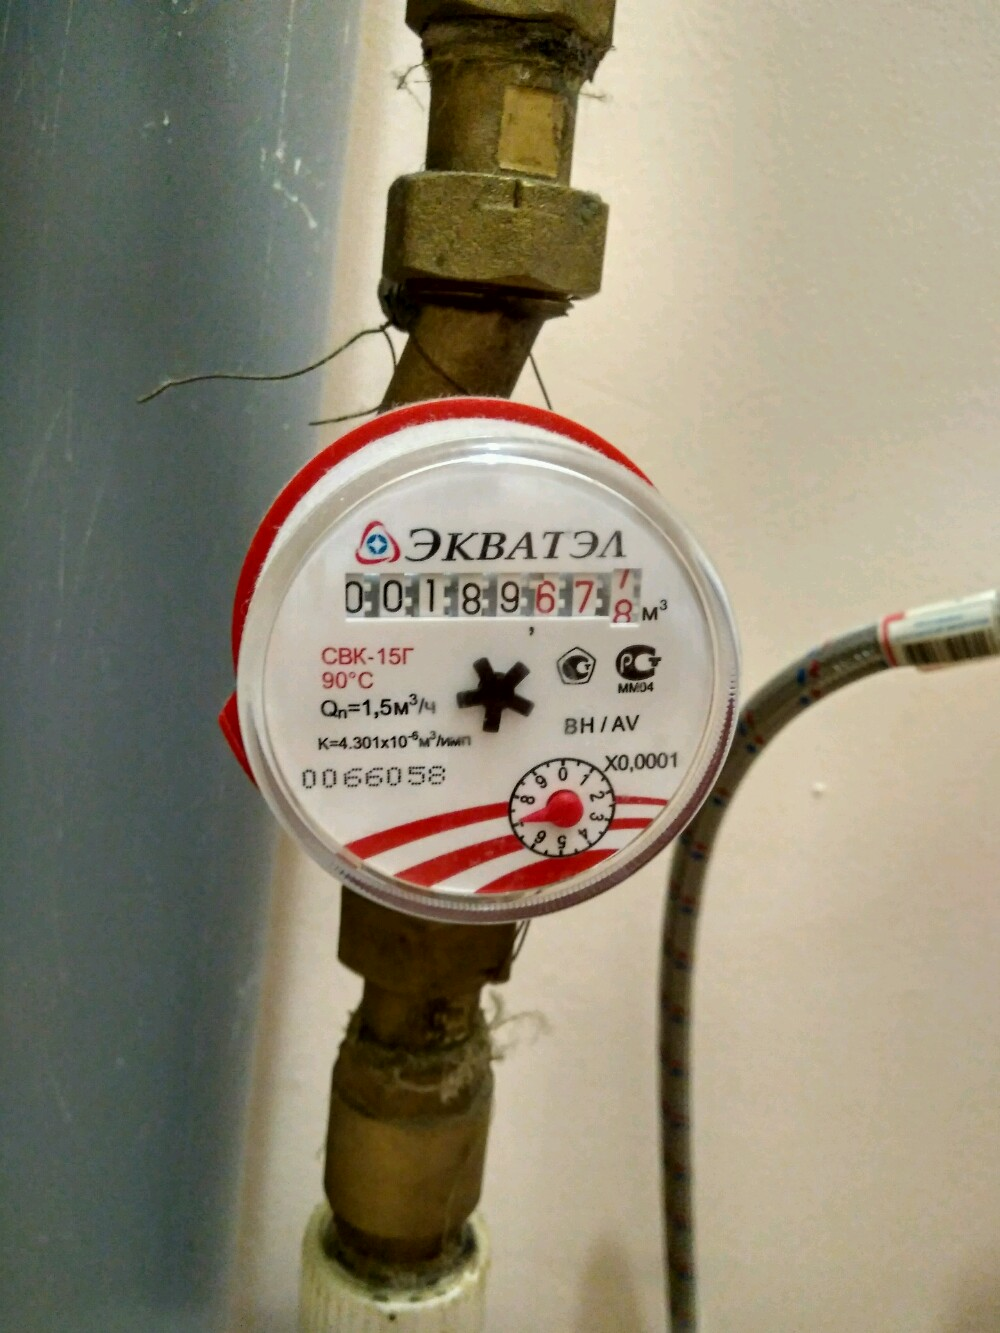
\includegraphics[width=\textwidth]{sections/imagens/Img_Original_Unet.jpg}
        \caption{Imagem Original}
        \label{fig:img1}
    \end{subfigure}\hfill % O \hfill fica colado no fechamento da primeira subfigura
    % Segunda Imagem
    \begin{subfigure}[b]{0.48\textwidth}
        \centering
        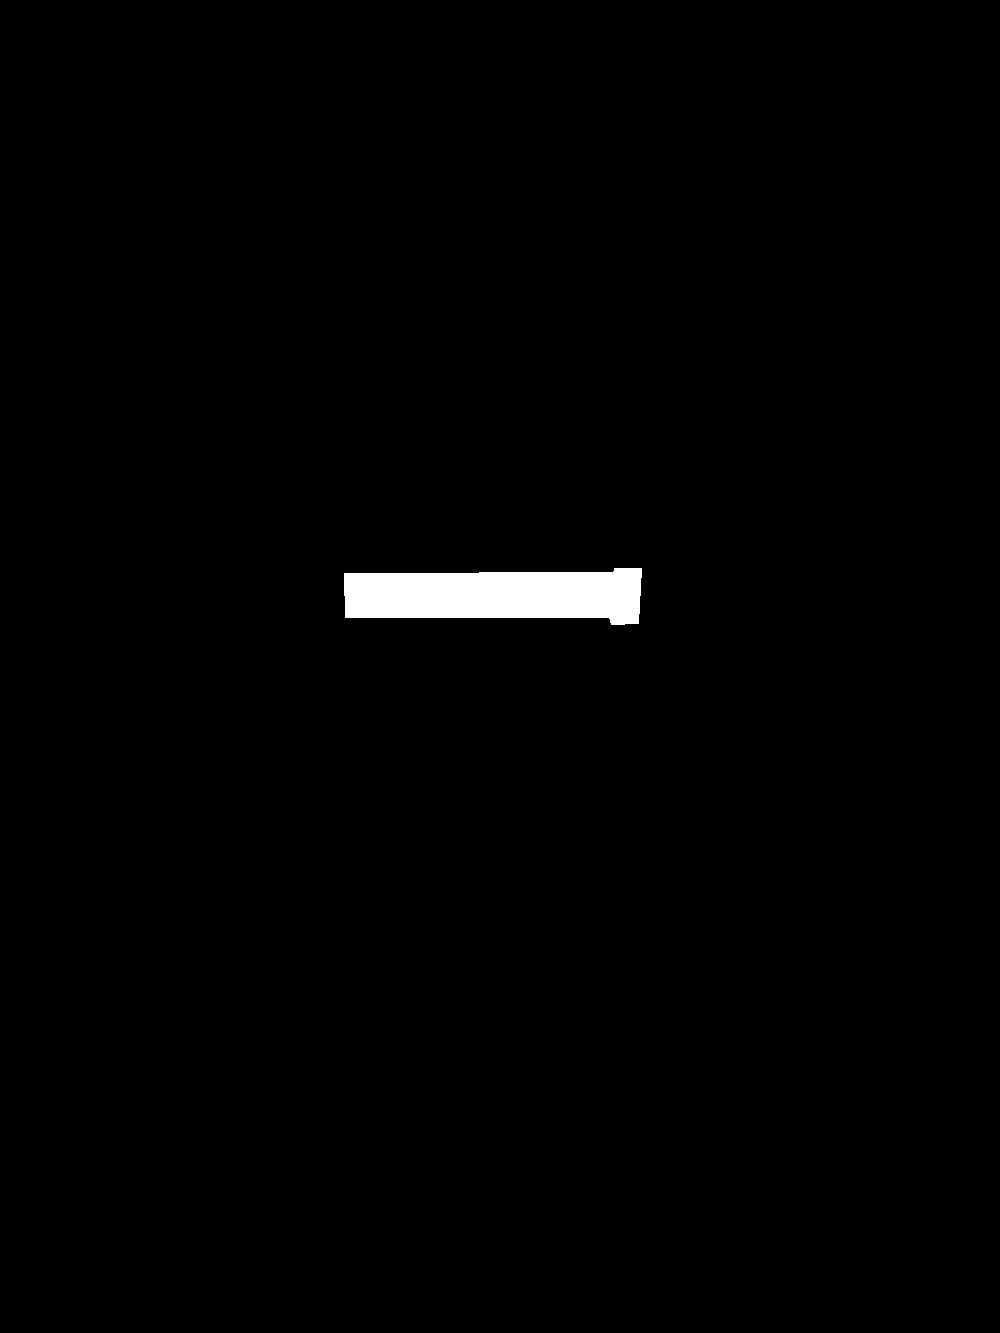
\includegraphics[width=\textwidth]{sections/imagens/Img_Mask_Unet.jpg}
        \caption{ROI Extraída da Imagem Original}
        \label{fig:img2}
    \end{subfigure}

    \fonte{Autores (2026).}
\end{figure}


A arquitetura U-Net é caracterizada pela presença de três etapas de 
processamento: Contração, Gargalo e Expansão. 
A camada de contração é composta por vários blocos, 
nos quais cada bloco recebe uma entrada e aplica uma camada de convolução seguida por 
uma camada de operação de max-pooling; essas camadas são matrizes 
que, respectivamente, apresentam a estrutura 3x3 e 2x2.

Com adendo, as camadas que constroem a arquitetura U-Net utilizam a função de ativação ReLU 
apresentada na equação~\ref{eq:relu_def}.

\begin{equation}
    f(x) = \text{ReLU}(x) = \max(0, x) = 
    \begin{cases} 
        x, & \text{se } x > 0 \\ 
        0, & \text{se } x \le 0 
    \end{cases}
    \label{eq:relu_def}
\end{equation}